
%(BEGIN_QUESTION)
% Copyright 2010, Tony R. Kuphaldt, released under the Creative Commons Attribution License (v 1.0)
% This means you may do almost anything with this work of mine, so long as you give me proper credit

An Allen-Bradley SLC 500 PLC is used to control a motor, using an across-the-line starter.  All 480 volt power wiring in this PLC-controlled ``bucket'' has been omitted for simplicity:

$$\includegraphics[width=15.5cm]{i02260x01.eps}$$

After many years of trouble-free operation, the motor refuses to start.  You have no test equipment with you -- all you have is what you see in the above illustration (with neither pushbutton pressed at the time).

\vskip 10pt

Identify the likelihood of each specified fault in this system.  Consider each fault one at a time (i.e. no coincidental faults), determining whether or not each fault could independently account for {\it all} observations and symptoms in this circuit.

% No blank lines allowed between lines of an \halign structure!
% I use comments (%) instead, so that TeX doesn't choke.

$$\vbox{\offinterlineskip
\halign{\strut
\vrule \quad\hfil # \ \hfil & 
\vrule \quad\hfil # \ \hfil & 
\vrule \quad\hfil # \ \hfil \vrule \cr
\noalign{\hrule}
%
% First row
{\bf Fault} & {\bf Possible} & {\bf Impossible} \cr
%
\noalign{\hrule}
%
% Another row
Open wire between Start switch and IN6 terminal &  &  \cr
%
\noalign{\hrule}
%
% Another row
Open wire between Stop switch and IN0 terminal &  &  \cr
%
\noalign{\hrule}
%
% Another row
Open contactor coil &  &  \cr
%
\noalign{\hrule}
%
% Another row
Shorted contactor coil &  &  \cr
%
\noalign{\hrule}
%
% Another row
Start switch incorrectly wired &  &  \cr
%
\noalign{\hrule}
%
% Another row
Failed input card &  &  \cr
%
\noalign{\hrule}
%
% Another row
Failed output card &  &  \cr
%
\noalign{\hrule}
%
% Another row
PLC program halted &  &  \cr
%
\noalign{\hrule}
%
% Another row
Blown fuse &  &  \cr
%
\noalign{\hrule}
} % End of \halign 
}$$ % End of \vbox

Finally, identify the {\it next} diagnostic test or measurement you would make on this system.  Explain how the result(s) of this next test or measurement help further identify the location and/or nature of the fault.

\vskip 20pt \vbox{\hrule \hbox{\strut \vrule{} {\bf Suggestions for Socratic discussion} \vrule} \hrule}

\begin{itemize}
\item{} Suppose we needed to perform some diagnostic tests on the Start and Stop switch input wiring which required actuating those switches repeatedly, but we did not want to actually start up the motor.  Explain how we could use the {\it force} utility in the PLC to accomplish this goal, and why it is very important we disable all of our imposed ``forces'' when the job is done.
\end{itemize}

\underbar{file i02260}
%(END_QUESTION)





%(BEGIN_ANSWER)


%(END_ANSWER)





%(BEGIN_NOTES)

% No blank lines allowed between lines of an \halign structure!
% I use comments (%) instead, so that TeX doesn't choke.

$$\vbox{\offinterlineskip
\halign{\strut
\vrule \quad\hfil # \ \hfil & 
\vrule \quad\hfil # \ \hfil & 
\vrule \quad\hfil # \ \hfil \vrule \cr
\noalign{\hrule}
%
% First row
{\bf Fault} & {\bf Possible} & {\bf Impossible} \cr
%
\noalign{\hrule}
%
% Another row
Open wire between Start switch and IN6 terminal &  & $\surd$ \cr
%
\noalign{\hrule}
%
% Another row
Open wire between Stop switch and IN0 terminal &  & $\surd$ \cr
%
\noalign{\hrule}
%
% Another row
Open contactor coil & $\surd$ &  \cr
%
\noalign{\hrule}
%
% Another row
Shorted contactor coil &  & $\surd$ \cr
%
\noalign{\hrule}
%
% Another row
Start switch incorrectly wired &  & $\surd$ \cr
%
\noalign{\hrule}
%
% Another row
Failed input card &  & $\surd$ \cr
%
\noalign{\hrule}
%
% Another row
Failed output card & $\surd$ &  \cr
%
\noalign{\hrule}
%
% Another row
PLC program halted &  & $\surd$ \cr
%
\noalign{\hrule}
%
% Another row
Blown fuse &  & $\surd$ \cr
%
\noalign{\hrule}
} % End of \halign 
}$$ % End of \vbox

\vskip 20pt \vbox{\hrule \hbox{\strut \vrule{} {\bf Virtual Troubleshooting} \vrule} \hrule}

This question is a good candidate for a ``Virtual Troubleshooting'' exercise.  Presenting the diagram to students, you first imagine in your own mind a particular fault in the system.  Then, you present one or more symptoms of that fault (something noticeable by an operator or other user of the system).  Students then propose various diagnostic tests to perform on this system to identify the nature and location of the fault, as though they were technicians trying to troubleshoot the problem.  Your job is to tell them what the result(s) would be for each of the proposed diagnostic tests, documenting those results where all the students can see.

During and after the exercise, it is good to ask students follow-up questions such as:

\begin{itemize}
\item{} What does the result of the last diagnostic test tell you about the fault?
\item{} Suppose the results of the last diagnostic test were different.  What then would that result tell you about the fault?
\item{} Is the last diagnostic test the best one we could do?
\item{} What would be the ideal order of tests, to diagnose the problem in as few steps as possible?
\end{itemize}

%INDEX% PLC, troubleshooting: motor start/stop control circuit

%(END_NOTES)

